\chapter{The lat_struct}
\label{c:lat.struct}
\index{lat_struct|hyperbf}

The \vn{lat_struct} is the structure that holds of all the information
about a lattice including any \vn{branch} and \vn{photon_branch} lines
(\sref{s:branch}). The components of a \vn{lat_struct} are listed in
Figure~\ref{f:lat.struct}.
\begin{figure}[htb]
\centering
\begin{verbatim}
type lat_struct
  character(16) name                       ! Name in USE statement
  character(40) lattice                    ! Lattice name
  character(80) input_file_name            ! Lattice input file name
  character(80) title                      ! From TITLE statement
  type (mode_info_struct)  a, b, z         ! tunes, etc.
  type (lat_param_struct) param            ! Lattice parameters
  type (ele_struct), pointer :: ele(:)     ! Array of lattice elements
  type (ele_struct) ele_init               ! For use by any program
  type (branch_struct), allocatable :: branch(:)   ! Branch arrays
  type (control_struct), allocatable :: control(:) ! control list
  type (coord_struct) beam_start           ! Starting coordinates.
  integer version                          ! Digested file version number
  integer n_ele_track                      ! elements in tracking lattice
  integer n_ele_max                        ! Index of last element used
  integer n_control_array                  ! last index used in control(:)
  integer n_ic_max                         ! last index used in ic(:) array
  integer input_taylor_order               ! As set in the input file
  integer, allocatable :: ic(:)            ! index to %control(:)
end type
\end{verbatim}
\caption{Definition of the \vn{lat_struct}.}
\label{f:lat.struct}
\end{figure}

\index{lat_struct!\%ele_init}
The \vn{%ele_init} component within the \vn{lat_struct} is not used
by \bmad and is available for general program use.


%----------------------------------------------------------------------------
\section{Pointers}
\label{s:lat:point}
\index{lat_struct!pointers}

Since the \vn{lat_struct} has pointers within it, there is an extra
burden on the programmer to make sure that allocation and deallocation
is done properly. To this end, the equal sign has been overloaded by
the routine \vn{lat_equal_lat} so that when one writes
\begin{example}
    type (lat_struct) lattice1, lattice2
    ! ... some calculations ...
    lattice1 = lattice2
\end{example}
the pointers in the \vn{lat_struct} structures will be handled
properly. The result will be that lattice1 will hold the same
information as \vn{lattice2} but the pointers in \vn{lattice1} will
point to different locations in physical memory so that changes to one
lattice will not affect the other.

\Hyperref{r:deallocate.lat.pointers}{deallocate_lat_pointers}
Initial allocation of the pointers in a \vn{lat_struct} variable is
generally handled by the \Hyperref{r:bmad.parser}{bmad_parser} 
and \Hyperref{r:lat.equal.lat}{lat_equal_lat}
routines.  Once allocated, local \vn{lat_struct} variables must have
the save attribute or the pointers within must be appropriately
deallocated before leaving the routine.
\begin{example}
  type (lat_struct), save :: lattice     ! Either do this at the start or ...
  ...
  call deallocate_lat_pointers (lattice) ! ... Do this at the end.
\end{example}
Using the save attribute will generally be faster but will use more
memory. Typically using the save attribute will be the best choice.

%----------------------------------------------------------------------------
\section{Branches in the lat_struct}
\label {s:lat.struct}

\index{lat_struct!\%branch(:)}
\index{branch}\index{photon_branch}\index{branch!root}
The lattice is divided up into the ``root branch'' 
(also called the ``root lattice'') and, if there are
\vn{branch} or \vn{photon_branch} elements, a number of other branches. 
To simplify the bookkeeping, the root lattice is itself considered a branch.

\index{branch_struct}
The branch information is contained in the \vn{%branch(0:)} array. The
\vn{%branch} array is always indexed from 0 with the $0$ branch
being the root branch.  The upper bound of this array will be equal to
the number of \vn{branch} plus \vn{photon_branch} elements present. The
definition of the \vn{branch_struct} structure is
\begin{example}
  type branch_struct
    character(40) name
    integer key                          ! photon_branch$, branch$, etc.
    integer ix_branch                    ! Index in lat%branch(:) array.
    integer ix_from_branch               ! 0 => root branch 
    integer ix_from_ele                  ! Index of branching element
    integer, pointer :: n_ele_track      ! Number of tracking elements
    integer, pointer :: n_ele_max
    type (ele_struct), pointer :: ele(:) ! Element array
    type (lat_param_struct), pointer :: param
  end type
\end{example}
\Hyperref{r:key.name}{key_name}
The \vn{branch(i)%key} component is set to either \vn{photon_branch\$}
or \vn{branch\$}. The \Hyperref{r:key.name}{key_name} function will
convert the integer key value to a string for printing. The value of the
\vn{%branch(i)%ix_branch} conponent is the branch index and will thus
have the value \vn{i}. This can be useful when passing a branch to a
subroutine.  The \vn{%branch(i)%ix_from_branch} component gives the
branch index of the branch that the $i$\Th branch branched off from.
\vn{%branch(i)%ix_from_ele} gives the index in the
\vn{%branch(j)%ele(:)} array of the \vn{branch} or \vn{photon_branch}
element that marks the beginning of the $i$\Th branch. Example:
\begin{example}
  type (lat_struct), target :: lat
  type (ele_struct), pointer :: ele
  ...
  ib = lat%branch(3)%ix_from_branch
  ie = lat%branch(3)%ix_from_ele
  ! ele is the branch or photon_branch element for lat%branch(3)
  ele => lat%branch(ib)%ele(ie)
  ! This is the same as the above.
  ele => pointer_to_ele(lat%branch(3)%ix_from_branch, lat%branch(3)%ix_from_ele)
\end{example}

Future plans include the simulation of multiple intersecting
machines. For example, a double ring collider. In this case,
individual branches could represent machines that are not connected.
To lessen the work needed to implement this plan, a branch that is not
connected to a prior branch has \vn{branch%ix_from_branch} set to
-1. Currently, only the root branch has \vn{branch%ix_from_branch} set
to -1.

\index{lat_struct!\%ele(:)}
\index{lat_struct!\%n_ele_track}
\index{lat_struct!\%n_ele_max}
\index{ele_struct!in lat_struct} 
\index{girder}
\index{overlay}
\index{group}
The \vn{%branch%ele(:)} array holds the array of elements in the
branch. Historically, the \vn{lat_struct} was developed at the start
of the \bmad project and branches were implemented well after that. To
maintain compatibility with older code, the \vn{lat%ele(:)} array, which
is used by older code, points to the same memory block as
the \vn{lat%%branch(0)%ele}
array. Similarly, \vn{%branch(0)%n_ele_track},
\vn{%branch(0)%n_ele_max}, and \vn{%branch(0)%param} point to
\vn{lat%n_ele_track}, \vn{lat%n_ele_max}, and \vn{lat%param} respectively.

The \vn{%branch%ele(:)} array is always allocated with zero as the
lower bound.  \vn{%ele(0)} is a marker element with its \vn{%name} component
set to ``\vn{BEGINNING}''. 
\vn{%ele(0)%mat6} is always the unit matrix. For the
root branch, the \vn{%branch(0)%ele(0:)} array is divided up into
two parts: The ``tracking'' part and a ``control'' part (also called
the ``lord'' part). The tracking part of this array holds the elements
that are tracked through. The control part holds elements that
control attributes of other elements (\sref{s:lat.control}). The bounds
of these two parts is given in Table~\ref{t:part.extent}.
\begin{table}[tb]
\begin{center}
\begin{tabular}{lll}
\toprule
              & \multicolumn{2}{c} {\em Element index}   \\ \cmidrule{2-3}
{\em section} & {\em min}          & {\em max}            \\ \midrule
tracking      & 0                  & \vn{%n_ele_track}    \\ 
control       & \vn{%n_ele_track}+1 & \vn{%n_ele_max}     \\ \bottomrule
\end{tabular} 
\caption[Bounds of the root branch array.]
{Bounds of the tracking and control parts 
of the root branch (\vn{lat\%branch(0)\%ele(:)}) array.}
\end{center}
\label{t:part.extent}
\end{table}
Only the root branch has a lord section so 
\vn{%branch%n_ele_track} and \vn{%branch%n_ele_max} are the same for 
all other branches. Since the root branch can also be accessed via the \vn{lat%ele(:)}
array, code that deals with the lord section of the lattice may use \vn{lat%ele(:)}
in place of \vn{lat%branch(0)%ele(:)}.

The index of the associated branch for a given \vn{branch} or
\vn{photon_branch} element is stored in \vn{%value(ix_branch_to\$)}:
\begin{example}
  ! Associated branch is: lat%branch(ix_branch)
  ix_branch = nint(branch_ele%value(ix_branch_to$))  
  direction = nint(branch_ele%value(direction$))
\end{example}
The direction will be +1 for forward branching and -1 for backward branching.

%----------------------------------------------------------------------------
\section{Param_struct Component}
\index{lat_param_struct}

The \vn{%param} component within each \vn{lat%branch(:)} is a
\vn{lat_param_struct} structure whose definition is shown in
Figure~\ref{f:lat.param.struct}
\begin{figure}[tb]
\centering
\begin{verbatim}
  type lat_param_struct
    real(rp) n_part             ! Particles/bunch (for beambeam elements).
    real(rp) total_length       ! total_length of lattice
    real(rp) unstable_factor    ! Circular lats: growth rate/turn. Linear lats: |orbit/limit|
    real(rp) t1_with_RF(6,6)    ! Full 1-turn 6x6 matrix
    real(rp) t1_no_RF(6,6)      ! Transverse 1-turn 4x4 matrix (RF off).
    integer particle            ! +1 = positrons, -1 = electrons
    integer ix_lost             ! If lost at what element?
    integer end_lost_at         ! entrance_end$ or exit_end$
    integer plane_lost_at       ! x_plane$, y_plane$, or z_plane\$
    integer lattice_type        ! linear_lattice$, circular_lattice$, etc...
    integer ixx                 ! Integer for general use
    logical stable              ! is closed lattice stable?
    logical aperture_limit_on   ! use apertures in tracking?
    logical lost                ! for use in tracking
  end type
\end{verbatim}
\caption{Definition of the \vn{param_struct}.}
\label{f:lat.param.struct}
\end{figure}

\index{lat_param_struct!\%total_length}
\vn{%param%total_length} is the length of the lattice that a beam
tracks through defined by
\begin{example}
  %param%total_length = %ele(n_ele_track)%s - %ele(0)%s
\end{example}
Normally \vn{%ele(0)%s} = 0 so \vn{%param%total_length} =
\vn{%ele(n_ele_track)%s} but this is not always the case.

\index{lat_param_struct!\%n_part}
\index{beambeam}
\index{lcavity!and param\%n_part}
\vn{%param%n_part} is the number of particles in a bunch and is used
by \vn{beambeam} element to determine the strength of the beambeam
interaction. \vn{%param%n_part} is also used by \vn{lcavity} elements
for wake field calculations.

\index{lat_param_struct!\%lost}
\index{lat_param_struct!\%ix_lost}
\index{lat_param_struct!\%end_lost_at}
\index{lat_param_struct!\%aperture_limit_on}
\index{lat_param_struct!\%plane_lost_at}
When tracking particles through a lattice the variable
\vn{%param%aperture_limit_on} determines if apertures are checked.
\vn{%param%lost} is used to signal if a particle is lost and
\vn{%param%ix_lost} gives the index of the element at which a particle
is lost. Additionally, \vn{%param%end_lost_at} is used to indicate at
which end the particle was lost at. Possible values for
\vn{%end_lost_at} are
\begin{example}
  %entrance_end
  %exit_end
\end{example}
The \vn{%plane_lost_at} component records whether
the lost particle was lost horizontally, vertically or longitudinally.
Possible values for \vn{%plane_lost_at} are
\begin{example}
  %x_plane
  %y_plane
  %z_plane
\end{example}
See Chapter~\ref{c:tracking} for more details.

\index{lat_param_struct!\%t1_with_RF}
\index{lat_param_struct!\%t1_no_RF}
\index{lat_param_struct!\%stable}
For circular lattices, \vn{%param%t1_with_RF} and \vn{%param%t1_no_RF}
are the 1--turn transfer matrices from the start of the lattice to the
end. \vn{%param%t1_with_RF} is the full transfer matrix with RF
on. \vn{%param%t1_no_RF} is the transverse transfer matrix with RF
off. \vn{%param%t1_no_RF} is used to compute the Twiss
parameters. When computing the Twiss parameters \vn{%param%stable} is
set according to whether the matrix is stable or not. If the matrix is
not stable the Twiss parameters cannot be computed. If unstable,
\vn{%param%unstable_factor} will be set to the growth rate per turn of
the unstable mode.

For linear lattices, if a particle is lost in tracking,
\vn{%param%unstable_factor} will be set to
\begin{example}
  orbit_amplitude / limit - 1
\end{example}

The particle type for a branch is stored in the
integer variable \vn{%param%particle}. The value of this variable will
correspond to one of the constants:
\index{positron\$}\index{electron\$}\index{proton\$}\index{antiproton\$}
\begin{example}
  positron\$
  electron\$
  proton\$
  antiproton\$
  photon\$
\end{example}
To print the name of the particle use the function
\vn{particle_name}. A particles mass and charge can be obtained from
the functions \vn{mass_of} and \vn{charge_of} respectively. 
\vn{charge_of} returns the particle's charge in units of $e$. Example:
\begin{example}
  type (lat_struct) lat
  ...
  print *, 'Beam Particles are: ', particle_name(lat%param%particle)
  if (lat%param%particle == proton\$) print *, 'I do not like protons!'
  print *, 'Particle mass (eV):    ', mass_of(lat%param%particle)
  print *, 'Particle charge:       ', charge_of(lat%param%particle)
\end{example}

%----------------------------------------------------------------------------
\section{Elements Controlling Other Elements}
\label{s:lat.control}

\index{lord|hyperbf}\index{slave|hyperbf}
In the \vn{lat_struct} structure, certain elements in the \vn{%ele(:)} 
array (equivalent to the \vn{%branch(0)%ele(:)} array),
called \vn{lord} elements, can control the attributes (component
values) of other \vn{%branch(:)%ele(:)} elements.  Elements so controlled are
called \vn{slave} elements.  The situation is complicated by the fact
that a given element may simultaneously be a \vn{lord} and a
\vn{slave}. For example, an \vn{overlay} element (\sref{c:control}) is
a lord since it controls attributes of other elements but an
\vn{overlay} can itself be controlled by other \vn{overlay} and
\vn{group} elements. In all cases, circular lord/slave chains are not permitted.

\index{ele_struct!\%lord_status}\index{ele_struct!\%slave_status}
The lord and slave elements can be divided up into classes. What type of
lord an element is, is set by the value of the element's
\vn{ele%lord_status} component. Similarly, what type of slave an element
is is set by the value of the element's \vn{ele%slave_status} component.
Nomenclature note: An element may be referred to by it's
\vn{%lord_status} or \vn{%slave_status} value. For example, an element
with \vn{ele%lord_status} set to \vn{super_lord\$} can be referred to as
a ``\vn{super_lord}'' element.

\index{free\$}\index{super_lord\$}
\index{group_lord}\index{girder_lord\$}
\index{multipass_lord\$}
\index{girder_lord\$}\index{not_a_lord\$}
The value of the \vn{ele%lord_status} component can be one of:
  \begin{description}
  \item[super_lord\$]\Newline 
A \vn{super_lord} element is created when elements are
superimposed on top of other elements (\sref{s:super}).
  \item[girder_lord\$]\Newline 
A \vn{girder_lord} element is a \vn{girder} element  (\sref{s:girder}). 
That is, the element will have \vn{ele%key} = \vn{girder\$}. In this
case, the slave elements are marked by setting the
\vn{slave_ele%on_a_girder} logical to \vn{True}.
  \item[multipass_lord\$]\Newline
\vn{multipass_lord} elements are created when
multipass lines are present (\sref{s:multipass}). 
  \item[overlay_lord\$]\Newline 
An \vn{overlay_lord} is an \vn{overlay} element (\sref{s:overlay}). 
That is, such an element will have \vn{ele%key} = \vn{overlay\$}.
  \item[group_lord\$]\Newline 
A \vn{group_lord} is a \vn{group} element (\sref{s:group}). That is,
such an element will have \vn{ele%key} = \vn{group\$}.
  \item[not_a_lord\$]\Newline
This element does not control anything.
  \end{description}
Any element whose \vn{%lord_status} is something other than
\vn{not_a_lord\$} is called a \vn{lord} element. In the \vn{tracking part}
of the lattice (\sref{s:lat.struct}), \vn{%lord_status} will always be
\vn{not_a_lord\$}. In the \vn{lord section} of the lattice, under normal
circumstances, there will never be any \vn{not_a_lord} elements.
However, it is permissible,
and sometimes convenient, for programs to set the \vn{%lord_status} of
a lord element to \vn{not_a_lord\$}.

\index{super_slave\$}\index{multipass_slave\$}
\index{patch_in_slave\$}\index{overlay_slave\$}
\index{group_slave\$}\index{free\$}\index{slice_slave\$}
The possible values for the \vn{ele%slave_status} component are:
  \begin{description}
  \item[free\$]\Newline
Free elements do not have any lord elements controlling them.
  \item[group_slave\$]\Newline
A \vn{group_slave} is an element that has one or more \vn{group_lord}
elements controlling the slave's attributes.  A \vn{group_slave} 
will not have any other types of lords.
  \item[multipass_slave\$]\Newline
A \vn{multipass_slave} element is the slave of a \vn{multipass_lord}
(\sref{s:multipass}).
  \item[overlay_slave\$]\Newline 
An \vn{overlay_slave} is an element that has one or more
\vn{overlay_lord} or \vn{girder_lord} lords. 
Note that an \vn{overlay_slave} can have
zero associated \vn{overlay_lord}s as long as it has a \vn{girder_lord}. 
Thus the term \vn{overlay_slave} is
a bit misleading. An \vn{overlay_slave} can also have associated
\vn{group_lord} elements.
  \item[patch_in_slave\$]\Newline
A \vn{patch_in_slave} is a \vn{patch} element that is also a
\vn{multipass_lord} with \vn{%ref_orbit} set to \vn{patch_out\$}
(\sref{s:multipass}). 
  \item[slice_slave\$]\Newline
A \vn{slice_slave} element represents a longitudinal slice of another element.
Slice elements are not part of the lattice but rather are created on-the-fly
when, for example, a program needs to track part way through an element.
  \item[super_slave\$]\Newline 
A \vn{super_slave} element is an element in the tracking part of the lattice that 
has one or more \vn{super_lord} lords (\sref{s:super}).
\end{description}

Any element whose \vn{%slave_status} is something other than
\vn{free\$} is called a \vn{slave} element. \vn{super_slave} elements
always appear in the tracking part of the lattice. The other types can
be in either the tracking or control parts of the lattice.

\begin{table}[tb]
  \footnotesize

  \centering
  \subfigure[Possible {ele\%lord_status} and {ele\%slave_status} combinations
    within an individual element.]
  {
 \begin{tabular}{lcccccc} 
    \toprule
    & \multicolumn{6}{c}{\vn{ele\%lord_status}} \\ \cmidrule{2-7}
    \vn{ele\%slave_status} &
    \begin{sideways}\vn{not_a_lord\$}\end{sideways} &
    \begin{sideways}\vn{group_lord\$}\end{sideways} &
    \begin{sideways}\vn{girder_lord\$}\end{sideways} &
    \begin{sideways}\vn{overlay_lord\$}\end{sideways} &
    \begin{sideways}\vn{multipass_lord\$}\end{sideways} &
    \begin{sideways}\vn{super_lord\$}\end{sideways}
    \\ \midrule
    %                           NL  GR  GI  O   M   S
    \vn{free\$}             & X & X & X & X & X & X \\ 
    \vn{group_slave\$}      & X & X & X & X & X & X \\ 
    \vn{overlay_slave\$}    & X & X & X & X & X & X \\ 
    \vn{patch_in_slave\$}   &   &   &   &   & X &   \\ 
    \vn{multipass_slave\$}  & X &   &   &   &   & X \\ 
    \vn{super_slave\$}      & X &   &   &   &   &   \\ \bottomrule
  \end{tabular}
  \label{f:lord.slave.a}
  }
  \hfill
  \subfigure[Possible {\%lord_status} and {\%slave_status} combinations
    for any lord/slave pair.]
  {
  \begin{tabular}{lcccccc} 
    \toprule
    & \multicolumn{6}{c}{\vn{lord\%lord_status}} \\ \cmidrule{2-7}
    \vn{slave\%slave_status} &
    \begin{sideways}\vn{not_a_lord\$}\end{sideways} &
    \begin{sideways}\vn{group_lord\$}\end{sideways} &
    \begin{sideways}\vn{girder_lord\$}\end{sideways} &
    \begin{sideways}\vn{overlay_lord\$}\end{sideways} &
    \begin{sideways}\vn{multipass_lord\$}\end{sideways} &
    \begin{sideways}\vn{super_lord\$}\end{sideways}
    \\ \midrule
    %                           NL  GR  GI  O   M   S
    \vn{free\$}             &   &   &   &   &   &   \\ 
    \vn{group_slave\$}      &   & X &   &   &   &   \\ 
    \vn{overlay_slave\$}    &   & X & X & X &   &   \\ 
    \vn{patch_in_slave\$}   &   &   &   &   & Y &   \\ 
    \vn{multipass_slave\$}  &   & 1 &   & X & X &   \\ 
    \vn{super_slave\$}      &   &   &   &   &   & X \\ \bottomrule
  \end{tabular}
  \label{f:lord.slave.b}
  }
  \caption[Possible element \%lord_status/\%slave_status combinations.]
  {Possible \%lord_status/\%slave_status combinations. 
   ``X'' marks a possible combination.
   ``1'' indicates that the slave will have exactly one lord of the type 
   given in the column. ``Y'' indicates the combination is not bidirectional.}
  \label{f:lord.slave}
\end{table}

\index{ele_struct!\%lord_status}\index{ele_struct!\%slave_status}
Only some combinations of \vn{%lord_status}
values and \vn{%slave_status} values are permissible for a given element.
Table~\ref{f:lord.slave.a} lists the valid combinations. Thus, for
example, it is {\em not} possible for an element to be simultaneously a
\vn{super_lord} and a \vn{super_slave}. 

\begin{figure}[tb]
\centering
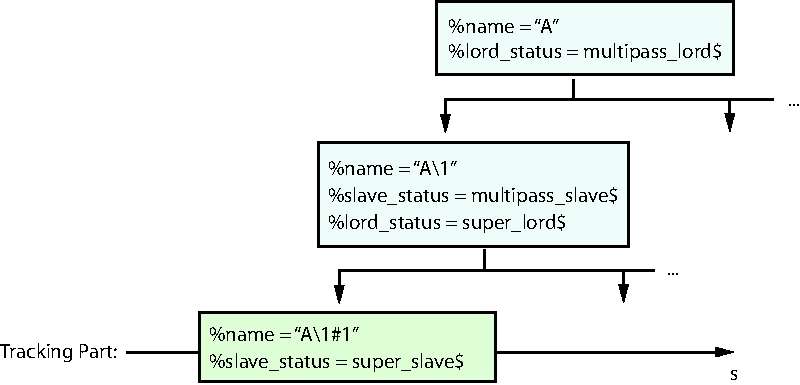
\includegraphics[width=5.5in]{super_multipass.pdf}
\caption[Example of multipass combined with superposition]
{Example of multipass combined with superposition. A \vn{multipass_lord}
element named \vn{A} controls a set of \vn{multipass_slaves} (only one shown).
The \vn{multipass_slave} elements are also \vn{super_lord} elements and they
will control \vn{super_slave} elements in the tracking part of the lattice.}
\label{f:super.mul}
\end{figure}

For lord/slave pairs,
Table~\ref{f:lord.slave.b} lists the valid combinations of
\vn{%lord_status} values in the lord element and \vn{%slave_status}
values in the slave element. Thus, for example, a
\vn{super_slave} may only be controlled by a \vn{super_lord}. In the
example in Section~\sref{s:multipass}, element \vn{A} would be a
\vn{multipass_lord} and \vn{A\B1} and \vn{A\B2} would be
\vn{multipass_slave}s. When superposition is combined with multipass,
the elements in the tracking part of the lattice will be
\vn{super_slave}s.  These elements will be controlled by
\vn{super_lord}s which will also be \vn{multipass_slave}s and these
\vn{super_lord}/\vn{multipass_slave} elements will be controlled by
\vn{multipass_lord}s. This is illustrated in Figure~\ref{f:super.mul}.

\index{ele_struct!\%n_lord}\index{ele_struct!\%n_slave}
The number of slave elements that a lord controls is given by the value
of the lord's \vn{%n_slave} component. Additionally, the number of lord
elements that the slave has is given by the value of the slave's.
\vn{%n_lord} component. To find the slaves and lords of a given element,
use the routines \Hyperref{r:pointer.to.slave}{pointer_to_slave} and
\Hyperref{r:pointer.to.lord}{pointer_to_lord}. Example:
\begin{example}
  type (lat_struct), target :: lat
  type (ele_struct), pointer :: this_ele, lord_ele, slave_ele
  ...
  this_ele => lat%ele(321)    ! this_ele points to a given element in the lattice

  do i = 1, this_ele%n_lord   ! Loop over all lords of this_ele
    ! lord_ele points to the i^th lord element of this_ele
    lord_ele => pointer_to_lord (this_ele, i)  
    ...
  enddo

  do i = 1, this_ele%n_slave  ! Loop over all slaves of this_ele
    ! slave_ele points to the i^th slave element of this_ele
    slave_ele => pointer_to_slave (this_ele, i) 
    ...
  enddo
\end{example}
The lord/slave bookkeeping is bidirectional. That is, 
for any given element, call it \vn{this_ele}, consider the
i\Th lord:
\begin{example}
  lord_ele_i => pointer_to_lord (this_ele, i)
\end{example}
then there will always be some index j such that the 
element pointed to by
\begin{example}
  pointer_to_slave(lord_ele_i, j)
\end{example}
is the original element \vn{this_ele}. The same is true for
the slaves of any given element. That is, for the i\Th slave
\begin{example}
  slave_ele_i => pointer_to_slave (this_ele, i)
\end{example}
there will always be some index j such that the 
element pointed to by
\begin{example}
  pointer_to_lord(slave_ele_i, j)
\end{example}
\index{patch_in_slave}
will be the original element \vn{this_ele}. 
The one exception here is that the lord of a
\vn{patch_in_slave} does not have a pointer back to
the \vn{patch_in_slave}.

\index{slave!ordering}\index{lords!ordering}
\index{super_lord}\index{super_slave}
\index{multipass_lord}\index{multipass_slave}
\index{patch_in_slave}
\index{patch}
The following ordering of slaves and lords is observed:
  \begin{description}
  \item[Slaves of a super_lord:] \Newline
The associated \vn{super_slave} elements of a given \vn{super_lord}
element are ordered from the entrance end of the \vn{super_lord}
to the exit end. That is, in the code snippet above,
\vn{pointer_to_slave (lat, this_ele, 1)} will point to the slave at
the start of the \vn{super_lord} and 
\vn{ pointer_to_slave (this_ele, this_ele%n_lord)}
will point to the slave at the exit end of the \vn{super_lord}.
  \item[Slaves of a multipass_lord:] \Newline
The associated \vn{multipass_slave} elements of a 
\vn{multipass_lord} element are ordered by pass number. That is, 
in the code snippet above, \vn{pointer_to_slave (this_ele, i)}
will point to the slave of the $i$\Th pass.
  \item[Lord of a multipass_slave:] \Newline
A \vn{multipass_slave} will have exactly one associated \vn{multipass_lord}
and this lord will be the first one. That is, 
\vn{pointer_to_slave (this_ele, 1)}.
  \item[Patch_in_slave:] \Newline
When a lattice input file has a \vn{patch} element that is used in a
multipass line and the \vn{patch} element has its \vn{ref_orbit}
attribute set to \vn{patch_out} (\sref{s:multi.patch}), the
\vn{multipass_lord} element corresponding to this element is also a
\vn{patch_in_slave}. In this case, the element will have exactly one
lord and that lord will be the \vn{multipass_lord} element corresponding
to the element specified by the \vn{ref_patch} attribute of the
\vn{patch_in_slave}. Using the example given in \sref{s:multi.patch},
the \vn{multipass_lord} corresponding to the \vn{p1} \vn{patch} element
will have a lord that is the corresponding element to the \vn{p2}
\vn{patch} element. The reason for this exception is so that the
slaves pointed to by \vn{pointer_to_slave} of a \vn{multipass_lord} 
will always be \vn{multipass_slave}s.
  \end{description}

\index{control_struct}
The element control information is stored in the \vn{lat%control(:)} array.
Each element of this array is a \vn{control_struct} structure 
\begin{example}
  type control_struct
    real(rp) coef                  ! control coefficient
    integer ix_lord                ! index to lord element
    integer ix_slave               ! index to slave element
    integer ix_branch              ! Branch index of the slave element.
    integer ix_attrib              ! index of attribute controlled
  end type
\end{example}
\index{girder}\index{overlay}\index{group}
\index{lat_struct!\%control}
Each element in the \vn{lat%control(:)} array holds the information on
one lord/slave pair. The \vn{%ix_lord} component gives the index of the
lord element which is always in the root branch --- branch 0. The
\vn{%ix_slave}  and \vn{%ix_branch} components give the element index
and branch index of the slave element. The \vn{%coef} and \vn{%ix_attrib}
components are used to store the coefficient and
attribute index for \vn{overlay} and \vn{group} control. The appropriate
control_struct for a given lord/slave pair can be obtained
from the optional fourth argument of the 
\Hyperref{r:pointer.to.lord}{pointer_to_lord} and
\Hyperref{r:pointer.to.slave}{pointer_to_slave} functions. 
Example: The following prints 
a list of the slaves, along with the attributes controlled and coefficients,
on all group elements in a lattice.
\begin{example}
  type (lat_struct), target :: lat
  type (ele_struct), pointer :: lord, slave
  type (control_struct), pointer :: con
  ...
  do i = lat%n_ele_track+1, lat%n_ele_max  ! loop over all lords
    lord => lat%ele(i) 
    if (lord%lord_status = group_lord$) then 
      print *, 'Slaves for group lord: ', lord%name
      do j = 1, lord%n_slave
        slave => pointer_to_slave (lord, j, ix_con)
        con => lat%control(ix_con)
        attrib_name = attribute_name (slave, con%ix_attrib)
        print *, i, slave%name, attrib_name, con%coef
      enddo
    endif
  enddo
\end{example}

\index{lat_struct!\%control}
\index{lat_struct!\%ix1_slave}\index{lat_struct!\%ix2_slave}
The elements in the \vn{lat%control(:)} array associated with
the slaves of a given lord are in the same order as the slaves and the 
index of the associated \vn{lat%control(:)} element of the first slave 
is given by the \vn{%ix1_slave} component of the lord
and the last slave is given by the \vn{%ix2_slave} component of the
lord. Example:
\begin{example}
  type (lat_struct), target :: lat
  type (ele_struct), pointer :: lord, slave
  ...
  lord => lat%ele(i)                    ! Point to some element
  if (lord%n_slave > 0) then
    slave => pointer_to_slave (lord, 1, ix_con)
    print *, lord%ix1_slave == ix_con   ! Will print "T" for True
    slave => pointer_to_slave (lord, lord%n_slave, ix_con)
    print *, lord%ix2_slave == ix_con   ! Will print "T" for True
  endif
\end{example}
This fact can be used to determine where a slave is in the list of slaves
for a lord. The following example prints the pass number of a \vn{multipass_slave}
taking advantage of the fact that the pass number 
\begin{example}
  type (lat_struct), target :: lat
  type (ele_struct), pointer :: lord, slave
  ...
  slave => lat%ele(i)                ! Point to some element  
  if (slave%slave_status == multipass_slave$) then
    ! The multipass_lord of this element is the first lord.
    lord => pointer_to_lord(slave, 1, ix_con)   
    print *, 'Multipass_slave: ', slave%name
    print *, 'Is in pass number:', ix_con - lord%ix1_slave + 1
  endif
\end{example}

\index{ele_struct!\%ic1_lord}\index{ele_struct!\%ic2_lord}
\index{lat_struct!\%ic}
Except for a \vn{slice_slave}, the \vn{%ic1_lord} and \vn{%ic2_lord} 
components of a given slave
element, along with the \vn{lat%ic(:)} array, can be used to find
the lords of the slave. 
Somewhat simplified, the code for the \xxx{pointer_to_lord} function is:
\begin{example}
  function pointer_to_lord (slave, ix_lord, ix_control) result (lord_ptr)
    implicit none
    type (lat_struct), target :: lat
    type (ele_struct) slave
    type (ele_struct), pointer :: lord_ptr
    integer, optional :: ix_control
    integer ix_lord, icon
    !
    icon = lat%ic(slave%ic1_lord + ix_lord - 1)
    lord_ptr => lat%ele(lat%control(icon)%ix_lord)
    if (present(ix_control)) ix_control = icon
  end function
\end{example}
This method for finding the lords of an element is considered
``private''. That is, no code outside of the official \bmad library
should rely on this.

%----------------------------------------------------------------------------
\section{Lattice Bookkeeping}
\label{s:lat.bookkeeping}

\index{reference energy}
The term ``lattice bookkeeping'' refers to the updating of
the appropriate parameter values when a given parameter in the lattice is
changed. For example, if the accelerating gradient of an \vn{lcavity}
element is modified, the reference energy parameter of all elements
downstream of the \vn{lcavity} will need to be changed and this can
also alter the transfer maps of the \vn{lcavity} and downstream
elements. \bmad divides the lattice bookkeeping into ``core'' part
and everything else. The core part itself is divided into five parts:
  \begin{description}
  \item[Attribute bookkeeping] \Newline
This refers to intra-element dependent attribute bookkeeping (\sref{s:depend}).
  \item[Control bookkeeping] \Newline
This refers to Lord/Slave bookkeeping for \vn{overlay}
(\sref{s:overlay}) and \vn{group} (\sref{s:group})elements, and for
\vn{superposition} (\sref{s:super}) and \vn{multipass}
(\sref{s:multipass}) lords.
  \item[Floor Position bookkeeping]
This refers to bookkeeping to keep track of an elements global ``floor'' position
stored in the \vn{ele%floor} structure.
  \item[Length bookkeeping]
This refers to bookkeeping to keep track of the longitudinal s-position of an element
stored in the \vn{ele%s} component.
  \item[Reference Energy bookkeeping]
This refers to the reference energy assigned to each element (\sref{s:ref.energy}).
\vn{ele%value(E_tot\$)} and \vn{ele%value(p0c\$)}
  \end{description}

\index{bookkeeping!automatic}
\index{bookkeeping!intelligent}
Historically, as the concept of lattice bookkeeping was being
developed, to be back compatible with existing programs, calls to
bookkeeping routines were added to calculational routines such as the
tracking routine \Hyperref{r:track1}{track1} and the routine for
calculating the linear transfer map \Hyperref{r:make.mat6}{make_mat6}.
This ``automatic'' bookkeeping system is inefficient since there is no
good way to keep track of what element attributes have been modified
which leads to redundant bookkeeping calculations. Eventually, as
\bmad developed and became more complicated, it was found that the
unnecessary bookkeeping load was generally causing a significant
slowdown in program execution time --- even in programs where no
element attributes were changed. To avoid this, an ``intelligent''
bookkeeping system was developed. In order to be back compatible with
existing programs, the automatic bookkeeping system is the
default. However, given the fact that the automatic bookkeeping system
has known deficiencies, and given the overhead with maintaining two
bookkeeping systems, the current plan is to start phasing out the
automatic bookkeeping system sometime in the not-so-far future. Thus
old programs should be converted to the new system and all new
programs should use the new bookkeeping system.

\index{bmad_common_struct!auto_bookkeeper}
To use intelligent bookkeeping, a program must set the global
\vn{bmad_com%auto_bookkeepper} to false. This is done once at the
start of the program. When a set of attributes needs to be modified,
the
\Hyperref{r:set.flags.for.changed.attribute}{set_flags_for_changed_attribute}
routine must be called for each element attribute that is set. After
all the attributes have been set,
\Hyperref{r:lattice.bookkeeper}{lattice_bookkeeper} is called to do
the core bookkeeping. Example
\begin{example}
  type (lat_struct) lat
  ...
  bmad_com%auto_bookkeeper = .false.    ! Only needs to be done once.
  ...
  lat%ele(i)%value(gradient$) = 1.05e6  ! Change, say, the gradient of an RFCavity
  call set_flags_for_changed_attribute (lat, lat%ele(i), lat%ele(i)%value(gradient$))

  ... Set attributes of other elements ...

  call lattice_bookkeeper (lat)         ! Do once after all attribute sets done.
\end{example}
The argument list for \vn{set_flags_for_changed_attribute} is 
\begin{example}
  set_flags_for_changed_attribute (lat, ele, attribute)
\end{example}
The \vn{attribute} argument may be either real, integer, or logical.

\index{ele!\%status}
\index{bookkeeper_status_struct}
The \vn{set_flags_for_changed_attribute} routine sets flags in the
\vn{ele%status} structure. This structure is of type
\vn{bookkeeper_status_struct} and looks like
\begin{example}
  type bookkeeper_status_struct
    integer attributes      ! Intra element dependent attribute status
    integer control         ! Lord/slave bookkeeping status
    integer floor_position  ! Global (floor) geometry status
    integer length          ! Longitudinal position status
    integer ref_energy      ! Reference energy status
    integer mat6            ! Linear transfer map status
    integer rad_int         ! Radiation integrals cache status
  end type
\end{example}
All components of this structure give the status of some lattice
bookkeeping aspect. The first five components of this structure
correspond to the five core bookkeeping parts discussed above. The
other two components are discussed below.

Possible values for the status components are
\begin{example}
  super_ok\$
  ok\$
  stale\$
\end{example}
The \vn{set_flags_for_changed_attribute} routine sets the appropriate
status components of an element to \vn{stale\$} which marks that
element for the appropriate bookkeeping. When the bookkeeping is done
by \vn{lattice_bookkeeper}, the \vn{stale\$} status components are set
to \vn{ok\$}. The \vn{super_ok\$} value is reserved for use by any
program that needs to do its own custom bookkeeping. How this works is
as follows: The \bmad bookkeeping routines will never convert a status
component with value \vn{super_ok\$} to \vn{ok\$} without first doing
some needed bookkeeping. Thus if a program sets a status component to
\vn{super_ok\$} and then later on finds that the status component is
set to \vn{ok\$}, the program knows that bookkeeping has been done. An
example will make this clear. Suppose a program needs to keep track of
a collection of high order transfer maps between various points in a
lattice. Suppose that the constant calculation of these maps would
slow the program done so it is desired to recalculate a given map only
when necessary. To implement this, the program could set the
\vn{ele%status%mat6} attribute of all the element to \vn{super_ok\$}
when the maps are calculated. If the program subsequently finds a
\vn{ele%status%mat6} attribute of an element set to \vn{ok\$} it knows
that it should recalculate any transfer maps that span that element.

It is guaranteed that when \vn{lattice_bookkeeper} is run,
all five core status components will not be \vn{stale\$}.
The routines used by \vn{lattice_bookkeeper} are:
\begin{example}
  \Hyperref{r:attribute.bookkeeper}{attribute_bookkeeper}      ! Intra-element attributes
  \Hyperref{r:control.bookkeeper}{control_bookkeeper}        ! Lord/slave control
  \Hyperref{r:s.calc}{s_calc}                    ! Longitudinal element s-position
  \Hyperref{r:lat.geometry}{lat_geometry}              ! Global (floor) positions.
  \Hyperref{r:lat.compute.reference.energy}{lat_compute_reference_energy}  ! Reference energy 
\end{example}
In general, these routines should not be called directly since the
correct way to do things is not always straight forward. See the code
for \vn{lattice_bookkeeper} for more details.

After the core bookkeeping is done, a program can call
\Hyperref{r:lat.make.mat6}{lat_make_mat6} to remake the transfer matrices.
\vn{lat_make_mat6} will remake the transfer matrices if either the
\vn{ele%status%mat6} flag is \vn{stale\$} or the reference orbit
around which the existing transfer matrix was computed has shifted.
\vn{lat_make_mat6} will set the \vn{ele%status%mat6} flag to \vn{ok\$}
for all elements whose transfer matrices are recomputed.

%---------------------------------------------------------------------------
\section{Finding Elements and Changing Attribute Values}
\label{s:lat.ele.change}

\index{ele_struct!\%ix_ele}
The routine \Hyperref{r:lat.ele.locator}{lat_ele_locator} 
can be used to search for an element
in a lattice by name or key type or a combination of both. Example:
\begin{example}
  type (lat_struct) lat
  type (ele_pointer_struct), allocatable :: eles(:)
  integer n_loc; logical err
  ...
  call lat_ele_locator ("quad::skew*", lat, eles, n_loc, err)
  print *, 'Quadrupole elements whose name begins with the string "SKEW":'
  print *, 'Name                 Branch_index        Element_index'
  do i = 1, n_loc  ! Loop over all elements found to match the search string.
    print *, eles(i)%ele%name, eles(i)%ele%ix_branch, eles(i)%ele%ix_ele
  enddo
\end{example}
This example finds all elements where \vn{ele%key} is \vn{quadrupole\$} 
and \vn{ele%name} starts with ``\vn{skew}''. See the documentation on 
\vn{lat_ele_locator} for more details on the syntax of the search string.

The \vn{ele_pointer_struct} array returned by \vn{lat_ele_locator} is
an array of pointers to \vn{ele_struct} elements
\begin{example}
  type ele_pointer_struct
    type (ele_struct), pointer :: ele => null()
  end type
\end{example}
The \vn{n_loc} argument is the number of elements found and the \vn{err} argument
is set True on a decode error of the search string.

Once an element (or elements) is identified in the lattice,
it's attributes can be altered. However, care must be taken that an element's attribute
can be modified (\sref{s:depend}). The function \vn{attribute_free} will
check if an attribute is free to vary.
\begin{example}
  type (lat_struct) lat
  integer ix_ele
  ...
  call lat_ele_locator ('Q10W', lat, eles, n_loc, err)   ! look for an element 'Q10W'
  free = attribute_free (eles(i)%ele, 'K1', lat, .false.)
  if (.not. free) print *, 'Cannot vary k1 attribute of element Q10W'
\end{example}

With user input the routine \vn{pointer_to_attribute} is a convenient
way to obtain from an input string a pointer that points to the
appropriate attribute. For example:
\begin{example}
  type (lat_struct) lat
  character(40) attrib_name, ele_name
  real(rp), pointer :: attrib_ptr
  real(rp) set_value
  logical err_flag
  integer ix_attrib, ie
  ...
  write (*, '(a)', advance = 'no') ' Name of element to vary: '
  accept '(a)', ele_name
  write (*, '(a)', advance = 'no') ' Name of attribute to vary: '
  accept '(a)', attrib_name
  write (*, '(a)', advance = 'no') ' Value to set attribute at: '
  accept *, set_value
  do ie = 1, lat%n_ele_max
    if (lat%ele(ie)%name == ele_name) then
      call pointer_to_attribute (lat%ele(ie), attrib_name, &
                            .false., attrib_ptr, ix_attrib, err_flag)
      if (err_flag) exit      ! Do nothing on an error
      attrib_ptr = set_value  ! Set the attribute
    endif
  enddo
\end{example}

changing an element attribute generally involves changing values in the 
\vn{%ele(i)%value(:)} array. This is done using the 
\vn{set_ele_attribute} routine. For example:
\begin{example}
  type (lat_struct) lat
  logical err_flag, make_xfer_mat
  ...
  call element_locator ('Q01W', lat, ix_ele)
  call set_ele_attribute (lat, ix_ele, 'K1', 0.1_rp, err_flag, make_xfer_mat)
\end{example}
\index{overlay}
This example sets the \vn{K1} attribute of an element named \vn{Q01W}.
\vn{set_ele_attribute} checks whether this element is actually free to
be varied and sets the \vn{err_flag} logical accordingly. An element's
attribute may not be freely varied if, for example, the attribute is
controlled via an \vn{Overlay}.

%----------------------------------------------------------------------------
\section{Beam_start Component}
\label{s:lat.beam.start}

\index{beam_start}
\index{lat_struct!\%beam_start}
The \vn{lat%beam_start} component is a \vn{coord_struct} structure for
holding the information obtained from \vn{beam_start} statements
(\sref{s:beam.start}) in a \bmad lattice file.

This component is not used in any standard \bmad calculation. It is up
to an individual program to use as desired.

%----------------------------------------------------------------------------
\section{Adding and Deleting Elements From a Lattice}
\label{s:lat.add.delete}

Modifying the number of elements in a lattice involves a bit of
bookkeeping. To help with this there are a number of routines. 

For adding elements there are three basic routines: To add a lord
element, the \Hyperref{r:new.control}{new_control} routine is used.  To add a new element
to the tracking part of the lattice, use the \Hyperref{r:insert.element}{insert_element}
routine. Finally to split an element into two pieces, the routine
\Hyperref{r:split.lat}{split_lat} is used. These basic routines are then used in such
routines as \Hyperref{r:create.overlay}{create_overlay} that creates overlay elements,
\Hyperref{r:create.group}{create_group} which creates group elements, \Hyperref{r:add.superimpose}{add_superimpose}
which superimposes elements, etc.

The routine \Hyperref{r:remove.eles.from.lat}{remove_eles_from_lat} is used to delete elements from
a lattice.


